\section{Introduction to the New Model}
This chapter introduces a new ``top-down'' Continuous and Proactive Security Assessment Model (CAPSAM) framework as a response to limitations in traditional risk assessment approaches. The case study by \citet{shaikh2023information} addressed the reactive nature of the Top Management Team (TMT)'s attention in its influence on the decision to carry out an Information Security Risk Assessment (ISRA). This reveals the need for a new proactive, continuous security model that integrates information security across all layers of an organisation.

\section{Overview of the CAPSAM Framework}
    \subsection{Purpose, Goals, and Intended Outcomes}
    The CAPSAM framework is designed to address the limitations of cybersecurity models by emphasising a proactive and continuous approach to risk assessment. Its primary purpose is to integrate information security considerations from the earliest stages of system development and throughout its lifecycle.

    The main goal of CAPSAM is to minimise the likelihood and impact of cybersecurity breaches through vigilant, ongoing risk management. The model aims to integrate information security across all layers of an organisation and focuses on continuous improvement, ensuring a resilient security posture that adapts to the ever-changing threat landscape. By doing this, CAPSAM prioritises the protection of all stakeholders\textemdash including the customer and their data\textemdash strengthening overall organisational security and trust.

    \subsection{The Five Pillars of CAPSAM}
    The core philosophies of CAPSAM can be summarised in five pillars: Culture, Continuous, Auditing, Response, Proactive (CCARP). These pillars are illustrated in Figure \ref{fig:CAPSAM_Pillars} and form the foundation of the model's approach to information security risk management.

    \begin{figure}[htbp]
        \centering
        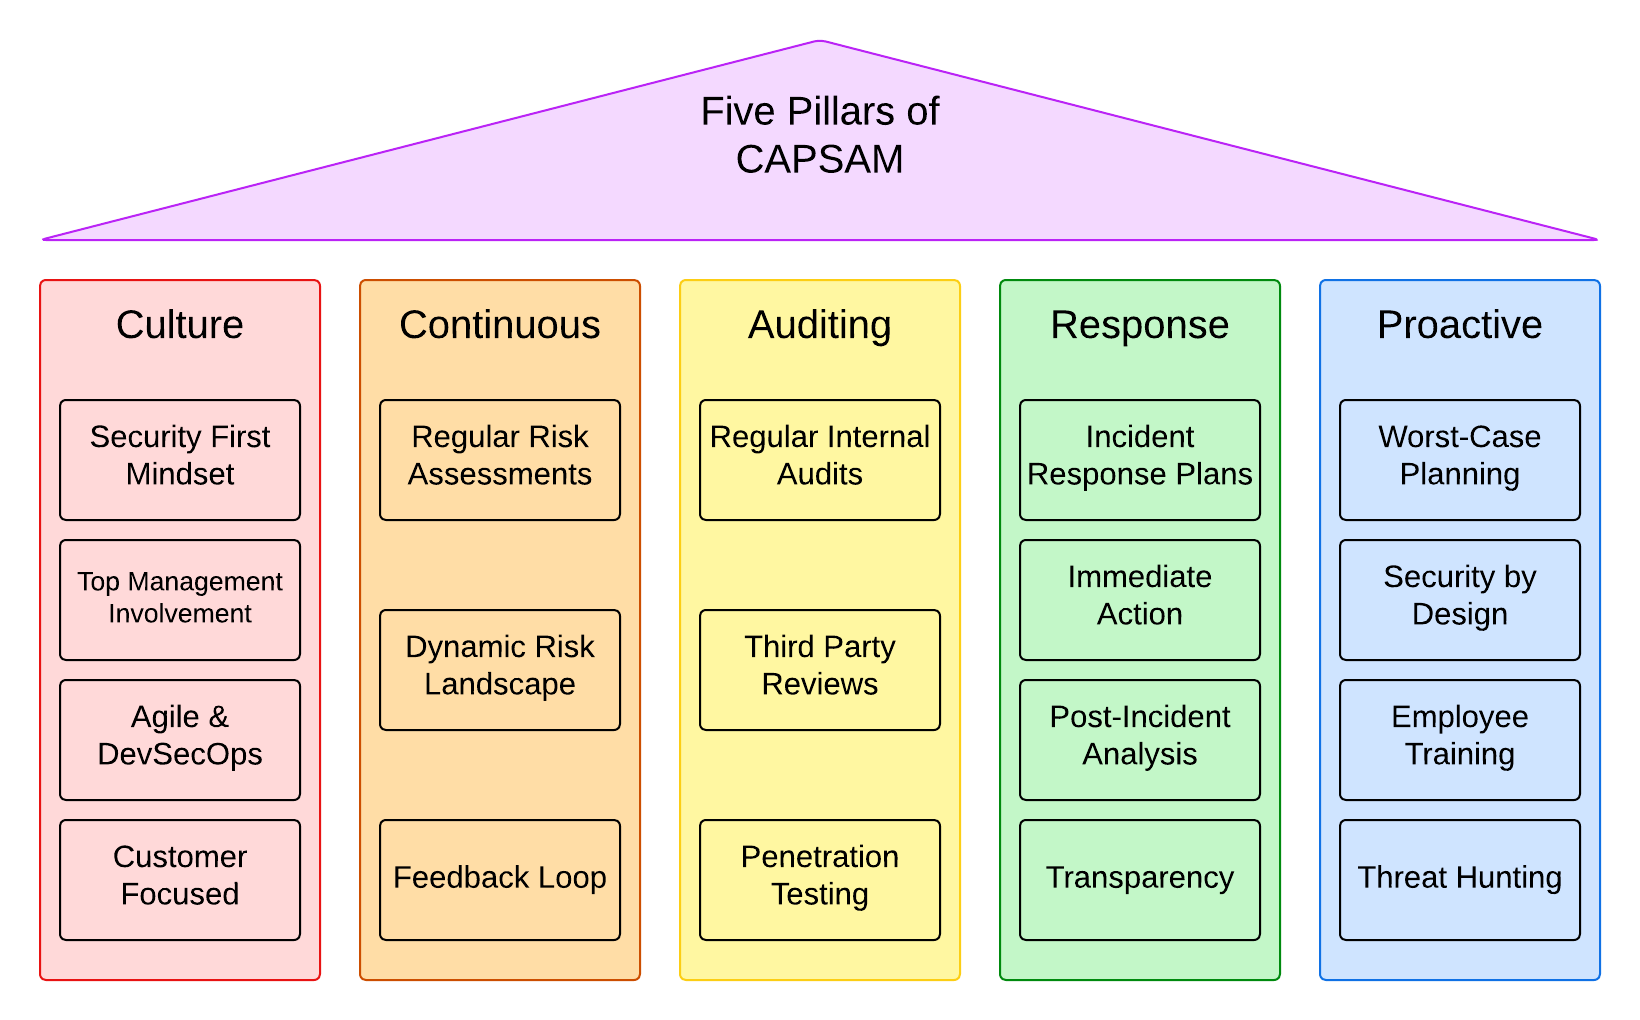
\includegraphics[width=0.8\textwidth]{figures/CAPSAM-Pillars.png}
        \caption{The Five Pillars of CAPSAM: Culture, Continuous, Auditing, Response, and Proactive (CCARP) and their components, explained in Table \ref{tab:CAPSAM_Pillars_Components} in appendices.}
        \label{fig:CAPSAM_Pillars}
    \end{figure}

    \subsection{FAMRM Cycle}
    The CAPSAM framework operates within the FAMRM cycle (New \textit{Feature}, Information Security Risk \textit{Assessment}, Proactive \textit{Mitigation} Strategies, Incident \textit{Response} Planning, and Continuous Threat \textit{Monitoring}). This cycle ensures that each new feature or system development is subject to proactive mitigation strategies, and continuous risk assessments where feedback loops inform the next ISRA. The FAMRM cycle is illustrated in Figure \ref{fig:FAMRM_Cycle}.

    \begin{figure}[htbp]
        \centering
        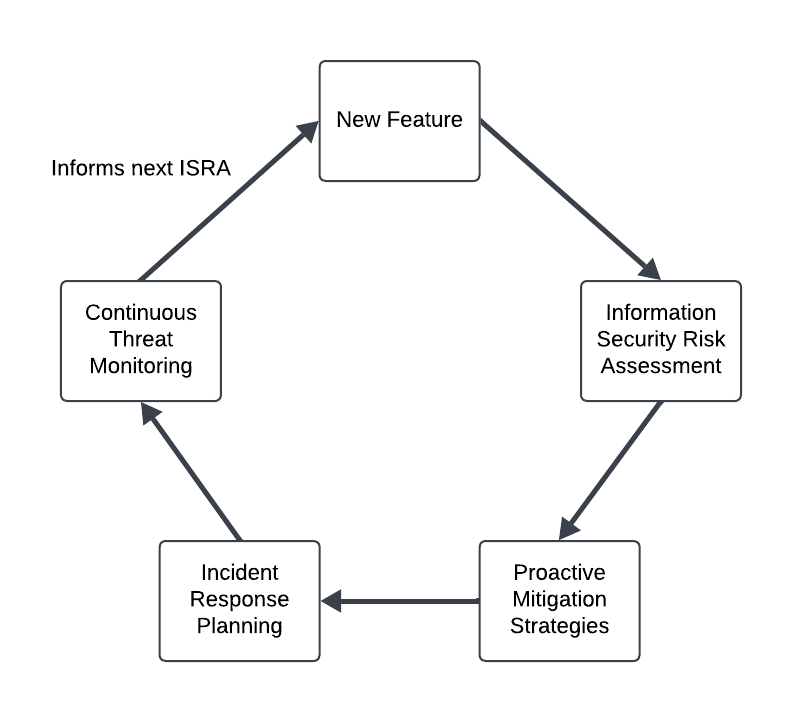
\includegraphics[width=0.6\textwidth]{figures/FAMRM-Cycle.png}
        \caption{FAMRM Cycle for Integrating Security into New Feature Development, Highlighting Continuous Risk Assessment, Proactive Mitigation, and Feedback Loops in Agile and DevSecOps Environments.}
        \label{fig:FAMRM_Cycle}
    \end{figure}

\section{Justification for a Top-Down Approach}
    \subsection{Establishing a Strong Security Posture through Executive Leadership}
    A top-down approach to information security risk management ensures strategic alignment and organisational commitment to security. By prioritising executive leadership, strategic priorities are set, resources allocated, and security policies enforced, framing information security as a core corporate governance issue rather than merely a technical concern \citep{linkov2014risk, fazlida2015information}. This alignment mirrors CAPSAM's emphasis on integrating security into organisational culture and fostering a ``security-first mindset'' among all stakeholders, as outlined in the `Culture' pillar.
    
    In contrast, bottom-up approaches focus on identifying technical vulnerabilities but often lack strategic direction, executive support, and adequate resource allocation \citep{fazlida2015information}. Without such oversight, efforts may neglect broader risks, including human and social factors, hindering a cohesive and effective security strategy \citep{shedden2010information}.
    
    \subsection{Corporate Governance and Strategic Integration}
    A top-down approach aligns with corporate governance by ensuring the Board of Directors (BOD) and executive management recognise their responsibility to safeguard information assets. \citet{fazlida2015information} explain that executive involvement integrates security into organisational strategies, enhancing competitive advantage, client satisfaction, and trust. This perspective aligns with CAPSAM's goal of embedding security considerations at all organisational levels, enabling seamless integration of security measures into daily operations. CAPSAM's FAMRM cycle, along with the `Culture' pillar, reinforce this integration by ensuring top management's active engagement and resource allocation.
    
    \subsection{Addressing the Limitations of Bottom-Up Approaches}
    Bottom-up approaches face significant challenges, including limited management buy-in and insufficient coordination across departments \citep{shaikh2023information}. This results in an overemphasis on technical controls while neglecting non-technical factors, such as human error and social engineering risks \citep{shedden2010information}. Furthermore, these strategies often fail to address the complex interactions of technical, social, and economic factors shaping an organisation's risk profile \citep{cai2017cybersecurity}. CAPSAM's top-down emphasis mitigates these issues by aligning policies with organisational needs and fostering a culture of security awareness through its `Culture' and `Proactive' pillars, ensuring holistic risk management.
    
\section{Theoretical Foundations}    
    \subsection{Attention-Based View (ABV) and CAPSAM's Culture Pillar}
    The Attention-Based View (ABV) theory highlights the importance of prioritising issues that are contextually relevant and salient \citep{shaikh2023information}. CAPSAM operationalises this theory by maintaining continuous focus on cybersecurity, thereby ensuring top management prioritises and allocates resources for proactive security measures. The `Culture' pillar reinforces this by securing top management involvement and embedding security as a core organisational value. This approach aligns with findings that management attention significantly increases the likelihood of conducting robust Information Security Risk Assessments (ISRAs) \citep{shaikh2023information}.
    
    \subsection{Agile and DevSecOps Principles in the Continuous Pillar}
    Agile methodologies and DevSecOps principles form a foundation for CAPSAM's `Continuous' pillar, promoting adaptability, speed, and integration of security into the development lifecycle \citep{ibm2021devsecops, dingsoyr2012agile}. Agile's iterative approach enables rapid adjustments to evolving threats, while DevSecOps emphasises visibility and auditability. The FAMRM cycle embodies these principles by incorporating ongoing risk assessments and iterative feedback loops, aligning security measures with the dynamic threat landscape \citep{ibm2021devsecops}.
    
    \subsection{ISO 31000: Risk Management Standard and the FAMRM Cycle}
    ISO 31000 provides a comprehensive framework for risk management, emphasising communication, monitoring, and continuous improvement \citep{purdy2010iso}. CAPSAM integrates these principles through the FAMRM cycle, ensuring a proactive and iterative approach to risk management. By focusing on dynamic assessments and mitigation strategies, CAPSAM addresses the limitations of static risk models, aligning with ISO 31000's definition of risk as the ``effect of uncertainty on objectives'' \citep{purdy2010iso}.
    
    \subsection{Organisational Learning and Feedback in CAPSAM}
    CAPSAM emphasises continuous learning through feedback loops, refining security measures based on insights from incident responses, audits, and risk assessments. This iterative approach, central to the FAMRM cycle, aligns with organisational learning principles advocating adaptation and sustained improvement \citep{murray2003continuous}. Regular audits and third-party reviews further support this dynamic model, enhancing resilience against evolving threats.
    
    \subsection{Trust and Customer-Focused Security}
    CAPSAM prioritises customer-focused security by embedding data protection at every stage of system development, reflecting stakeholder theory and corporate social responsibility (CSR) principles \citep{moir2001csr, parmar2010stakeholder}. The Culture pillar's emphasis on transparency and proactive incident response aligns with trust theory, which underscores the role of organisational credibility in fostering stakeholder trust \citep{castelfranchi2010trust}. Trust is treated as relational capital, benefiting both the organisation and its stakeholders by enhancing credibility and reliability \citep{castelfranchi2010trust}.      

\section{Critical Analysis of CAPSAM}
    \subsection{Strengths of CAPSAM}
    CAPSAM stands out due to its proactive nature, allowing organisations to address potential threats before they manifest, thus reducing the likelihood of successful cyberattacks. It fosters a ``security-first mindset'', ensuring security is a shared responsibility across the organisation. By integrating security into agile development cycles and DevSecOps practices, CAPSAM supports iterative, security-conscious development. Its continuous improvement cycle, driven by ongoing risk assessments and feedback loops, ensures that security remains robust in the face of emerging threats. Additionally, CAPSAM's focus on customer data protection builds trust by embedding security throughout the system development process.

    \subsection{Limitations of CAPSAM}
    Despite its advantages, CAPSAM presents several challenges. The model requires continuous updates to risk assessments, which can be resource-intensive. Ongoing monitoring demands significant resources and may lead to over-reliance on specific teams or individuals. CAPSAM's success hinges on top management's commitment to allocating resources for cybersecurity, which can be a hurdle. Regular internal audits and third-party reviews, including penetration testing, are necessary but can be time-consuming and require external expertise. Consistent application of CAPSAM's principles in large organisations can also prove difficult \citep{purdy2010iso}.

    \subsection{Comparison with Case Study Approach}
    CAPSAM's proactive approach contrasts with the reactive strategy of the case study, which focuses on addressing issues after a breach has occurred. CAPSAM integrates security from the earliest stages of development, embedding it across all organisational levels. In contrast, reactive approaches often prioritise technical fixes without addressing underlying managerial issues \citep{shedden2010information, shaikh2023information}. CAPSAM's continuous nature allows for dynamic responses to emerging threats, while reactive methods are limited to incident response and do not ensure long-term resilience. By addressing vulnerabilities early and continuously, CAPSAM avoids many issues seen in reactive models.

    \subsection{Challenges in Implementing CAPSAM}
    Implementing CAPSAM requires securing top management support to allocate resources and prioritise cybersecurity as a strategic objective \citep{shedden2010information}. \citet{fazlida2015information} highlight that gaining board of directors (BOD) support can be difficult, as cybersecurity is often viewed solely as an IT issue, with some boards lacking the expertise to address risks and being overwhelmed by ``technical jargon'' \citep{hartmann2021academic}. CAPSAM also necessitates consistent cross-department communication, ongoing training, and significant resources for continuous monitoring, including staffing and tools. Overcoming resistance to change from those accustomed to reactive approaches is another challenge \citep{murray2003continuous}, and regular audits and penetration tests require additional expertise and time.

\section{Implementation of CAPSAM}
    \subsection{Phase 1: Planning and Preparation}
    The first phase involves securing commitment from top management to allocate resources and prioritise cybersecurity as a core strategic objective. It is essential to conduct an initial risk assessment, identify stakeholders, define roles and responsibilities, and establish clear communication channels. Aligning the security risk management policy with the organisation's overall strategy ensures that security is integrated into the organisation's broader objectives. This phase also involves fostering a cultural shift towards security and collaboration across departments, breaking down silos and encouraging organisation-wide engagement.

    \subsection{Phase 2: Implementation}
    In this phase, organisations adopt a DevSecOps approach, integrating security throughout the software development lifecycle. Organisations conduct risk assessments to identify vulnerabilities, prioritise risks, and develop mitigation strategies. Security must be addressed from the start and continuously monitored to maintain a proactive security posture. Mitigation strategies should be implemented to manage identified risks, and regular training should be provided to ensure employees understand their role in managing security risks, reinforcing a shared responsibility across the organisation.

    \subsection{Phase 3: Review and Improvement}
    The final phase focuses on regular assessments to review the effectiveness of CAPSAM and adapt it based on insights from risk assessments, incident responses, and business changes. This phase promotes continuous improvement, ensuring that the system’s security posture evolves to meet emerging threats. Additionally, fostering a culture of ongoing vigilance and collaboration is essential to ensure that security remains a core value across the organisation, preventing a return to siloed working.